
\section{Effective Acceptance} \label{EffectiveAcceptanceSection}

%% Definition 
After the event number is determined by the template fit, the next important ingredient to calculate the antiproton to proton flux ratio is the effective acceptance.    \par

For a spectrometer, the counting rate of a given particle species depends on the flux intensity and the geometrical acceptance $A_\mathrm{geo}$ \cite{SULLIVAN19715}. The geometrical acceptance is a fixed value for a certain apparatus, but this assumes no interaction between the traversing particles and the apparatus, while for data analysis, dedicated cuts and selections are applied. Therefore, considering this, the geometrical acceptance is multiplied by the efficiencies of the cuts and the selections $\epsilon_\mathrm{cut}$. This product is called effective acceptance $A_\mathrm{eff}$. The larger the effective acceptance, the more events can be collected. \par

\begin{equation}
\label{EffectiveAcceptanceDefination}
A_\mathrm{eff}=A_\mathrm{geo} \times \epsilon_\mathrm{cut} 
\end{equation}

%% Calculating acceptance: Acceptance in AMS-02
Calculating the effective acceptance directly is impossible. The practical way is to use the MC simulation method. In the AMS-02 experiment, different MC production models with the help of Geant4 are widely used. In these models, the whole detector is located inside a cube with an edge length of 3.9 m. To mimic an isotropic flux, the generated artificial particles are continuously emitted on the plane defined by the cube side that lies on the top of the detector, and randomly go down with a solid angle of $\pi \cdot \rm{sr}$.  \par
%The generated momentum spectrum follows either a power law with a spectrum index equal to -2.7 or it is constant as a function of log($p$). \par

According to \cite{SULLIVAN19715}, the acceptance can be calculated with two ingredients: the number of passed events $N_\mathrm{pass}$ and the number of generated events above the top plane $N_\mathrm{generated}$. The formula is given in equation \ref{AcceptanceCalculation}. For the calculation of effective acceptance, apart from the geometry of the detectors, the cut efficiency also reduces the number of passed events.

\begin{equation}
\label{AcceptanceCalculation}
A_\mathrm{eff}=\pi \cdot A \cdot \frac{N_\mathrm{passed}(R_\mathrm{true})}{N_\mathrm{generated}(R_\mathrm{true})}
\end{equation}        
where A=3.9 $m$ $\cdot$ 3.9 $m$. \par

%% P and Pbar acceptance different:cross section
Because the interaction cross sections for proton on carbon and aluminum are different from the cross sections for antiproton on carbon and aluminum especially in the low rigidity range \cite{PbarCrossSection1, PbarCrossSection2, ProtonCrossSection1, ProtonCrossSection2}, this difference results in different effective acceptance for proton and antiproton in this analysis, and therefore proton effective acceptance $A_{p}$ to antiproton effective acceptance $A_{\bar{p}}$ ratio is not equal to one. In figure \ref{EffectiveAcceptance}, the effective acceptances of proton and antiproton are given. \par


\begin{figure}[htbp]
    \centering
    \subfigure[]{
        \includegraphics[width=0.505\textwidth, trim=0cm 0cm 0.7cm 0cm, clip ]{Figures/chapter4/Acceptance/EffectiveAcceptance/{Acceptance_Proton}.pdf} %xleftupper, yleftbottom, xrightbottom, yrightupper

    }
    \hspace{-1cm}
    \subfigure[]{
	\includegraphics[width=0.505\textwidth, trim=0cm 0cm 0.7cm 0cm, clip]{Figures/chapter4/Acceptance/EffectiveAcceptance/{Acceptance_Antiproton}.pdf} 
    } 
    %\vspace{-3mm}
    \caption[Effective acceptance of protons and antiprotons.]{Effective acceptance of a) proton and b) antiproton in different rigidity ranges. In the low and intermediate range, the inner central tracker pattern is used. In the high rigidity range, the FullSpan, Inner+L1, Inner+L9 and Inner Only tracker patterns are used. Due to different selections in different rigidity ranges, the effective acceptances are determined individually.} 
    \label{EffectiveAcceptance}
\end{figure}


%% Data/MC correction (Acceptance in Pbar Ratio Study)
\begin{figure}[htbp]
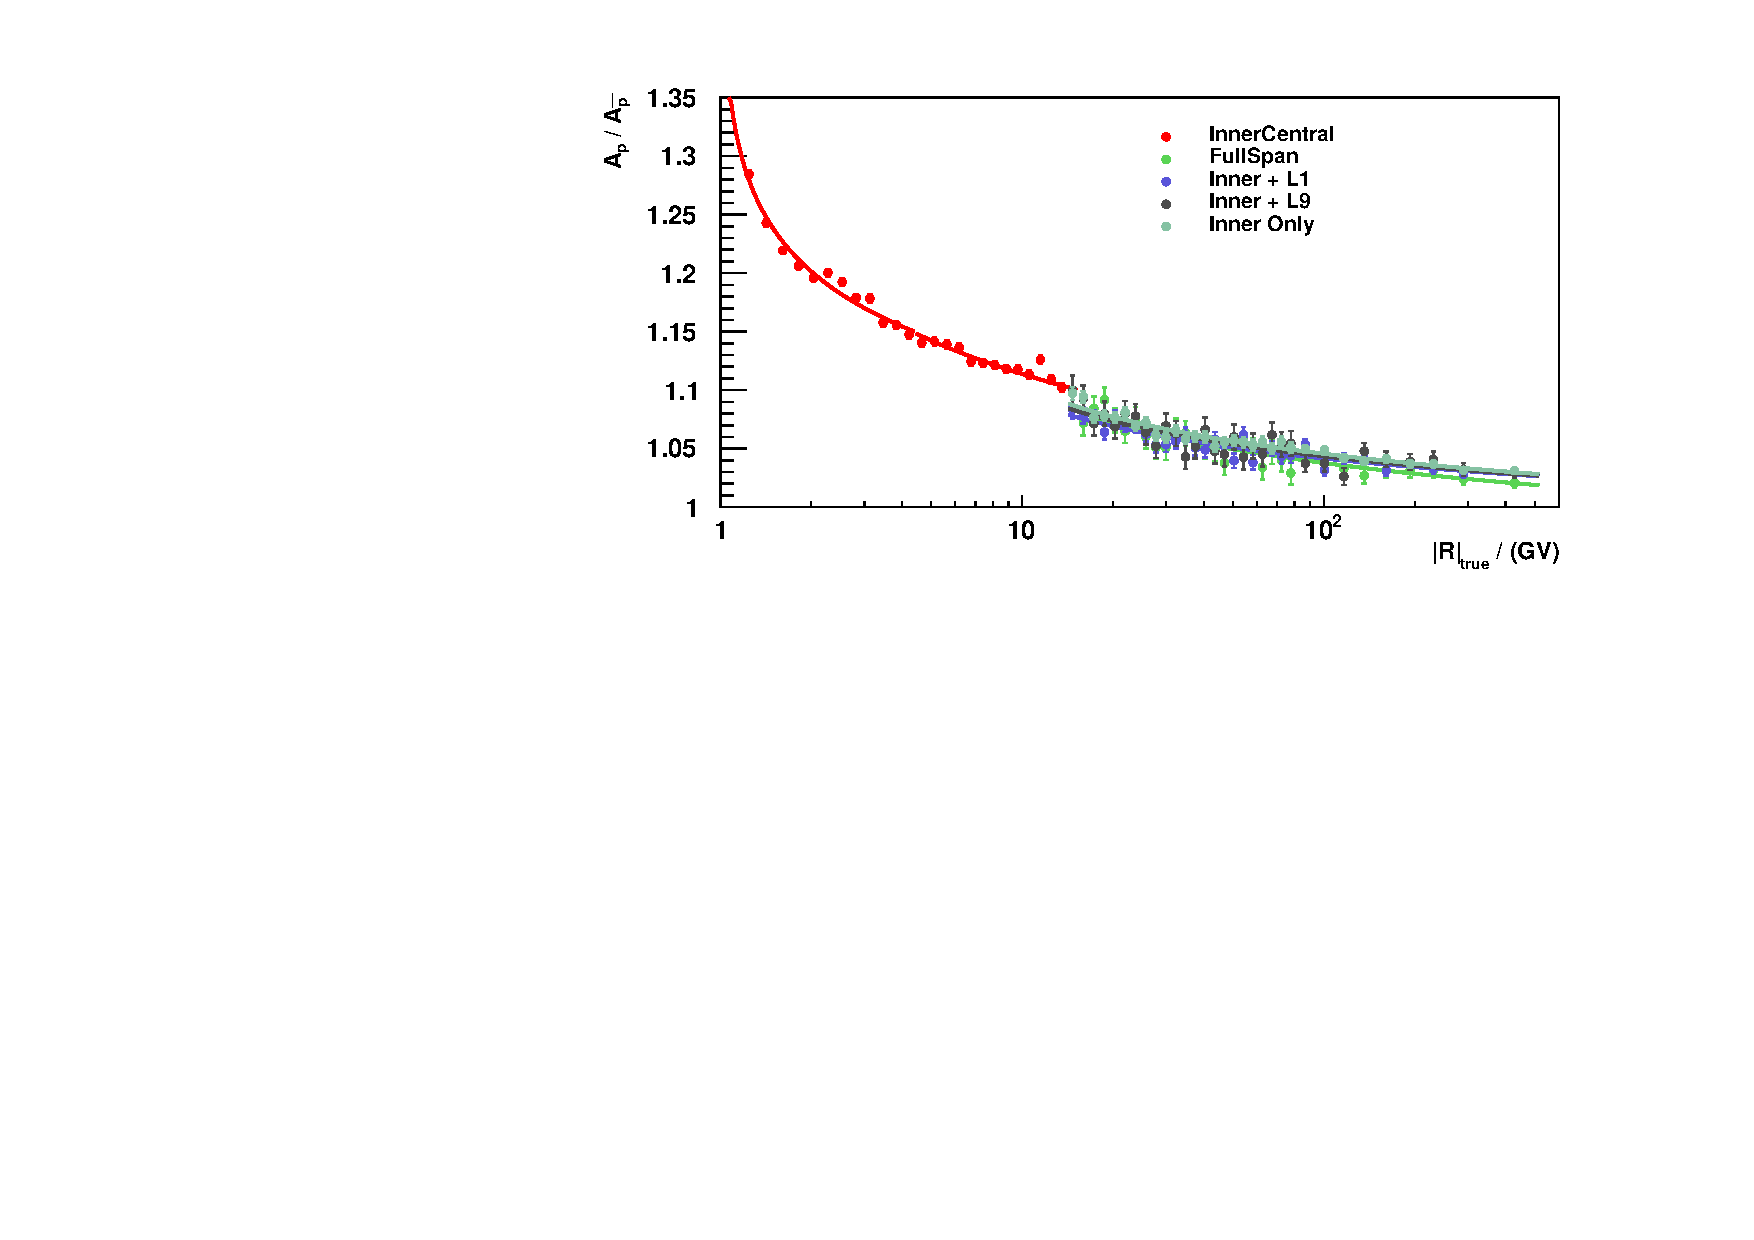
\includegraphics[width=1.00\textwidth]{Figures/chapter4/Acceptance/EffectiveAcceptanceRatio/AcceptancePlot.pdf}
\caption[Proton to antiproton effective acceptance ratios.]{Proton to antiproton effective acceptance ratios in different rigidity ranges. Due to the different selections and tracker patterns, the effective acceptance ratios are calculated individually. The uncertainty in this plot is statistical uncertainty only, the uncertainty due to the cross section will be discussed in Section \ref{SystematicUncertaintiesSection}. To have a smooth curve of the effective acceptance ratio, parameterizations are used.}
\label{TheEffectiveAcceptanceRatio}
\end{figure}

The effective acceptance ratio is rigidity-dependent and it is taken from MC first. Due to differences between ISS data and MC simulation, the effective acceptance obtained from MC needs to be corrected with the data/MC efficiency ratio. Since both of the MC determined proton effective acceptance $A^\mathrm{MC}_{p}$ and antiproton effective acceptance $A^\mathrm{MC}_{\bar{p}}$ need data/MC correction, namely $\delta_{p}$ and $\delta_{\bar{p}}$. This correction is assumed to be canceled out strictly. The same effect is valid also in the positron/electron ratio analysis \cite{ZimmermannPhDThesis}. Therefore, the effective acceptances ratio can be purely determined by MC simulations. \par

\begin{equation}
\label{EffectiveAcceptanceRatioCanceledOut}
%\frac{\Phi_{\bar{p}}}{\Phi_{p}} = \frac{N_{\bar{p}}}{N_p} \cdot \frac{A_{p}}{A_{\bar{p}}} = \frac{N_{\bar{p}}}{N_p} \cdot \frac{A^{MC}_{p}}{A^{MC}_{\bar{p}}} \cdot \frac{1+\delta_{p} }{1+ \delta_{\bar{p}} } = \frac{N_{\bar{p}}}{N_p} \cdot \frac{A^{MC}_{p}}{A^{MC}_{\bar{p}}}
\frac{A_{p}}{A_{\bar{p}}} = \frac{A^\mathrm{MC}_{p}}{A^\mathrm{MC}_{\bar{p}}} \cdot \frac{1+\delta_{p} }{1+ \delta_{\bar{p}} } = \frac{A^\mathrm{MC}_{p}}{A^\mathrm{MC}_{\bar{p}}}
\end{equation}     

Due to the different selections and different tracker patterns in three rigidity ranges, the proton to antiproton effective acceptance ratios are slightly different and determined individually. In figure \ref{TheEffectiveAcceptanceRatio}, the antiproton to proton effective acceptance ratio is shown. To avoid fluctuations in the effective acceptance ratios, the parameterizations of the effective acceptance ratios are done in different ranges individually.







